% Welche Datenbank wurde verwendet und warum,...
\subsection{Anforderungen}
\paragraph{}
Es wird eine moderne Plattform entwickelt, auf der sich Nutzer ähnlich Social Media Profile anderer Nutzer anschauen und miteinander Chats führen. Nutzer sollen in Echtzeit miteinander schreiben können und nahezu keine Wartezeit in Kauf nehmen müssen, um sich andere Profile anzeigen zu lassen. Die Datenbank muss nahezu immer erreichbar sein, da unsere Webseite ohne Datenbankanbindung nur beschränkt nutzbar ist. Um eine potenziell große Anzahl an Nutzern in der Zukunft des Projektes verwalten zu können, sollte es angemessene Skalierungsmöglichkeiten geben.

\paragraph{}
Im Folgenden gehen wir näher auf die Ziele der Datenbank ein und vergleichen die NoSQL Datenbank MongoDB mit PostgreSQL, welche repräsentativ für SQL basierte ORDBMS steht. 

\subsubsection{Lese- und Schreibgeschwindigkeit}
\paragraph{}
Um eine möglichst gute Benutzerfahrung zu gewährleisten, wird versucht, die Wartezeit beim Laden der Webseite zu verringern.\\
Eine Möglichkeit dafür ist eine optimistische Benutzeroberfläche. Bei dieser wird davon ausgegangen, dass der angefragte Schreibzugriff erfolgreich ist; dem Nutzer wird bereits visuell der Erfolgsfall angezeigt. Sollte der Schreibzugriff fehlschlagen,  wird der Status der Benutzeroberfläche zurückgesetzt und der Nutzer durch eine Fehlermeldung informiert. Im Gegensatz zu einer realistischen Benutzeroberfläche, welche sich erst aktualisiert, wenn die Datenbank antwortet und der Schreibzugriff genehmigt wurde, erhält der Benutzer sofort eine Rückmeldung und muss nicht auf eine Antwort unseres Servers warten.\\
Anders als Schreibanfragen, welche mit einer Bestätigung oder Ablehung der Anfrage antworten, fordern Leseanfragen Daten an. Wartezeiten bei Leseanfragen können daher nicht maskiert werden.\\
Um in einem späteren Entwicklungsschritt die Reduzierung der Wartezeiten durch eine optimistische Benutzeroberfläche zu ermöglichen, werden daher langsamere Schreibgeschwindigkeiten in Kauf genommen, wenn sich mit dieser Entscheidung die Lesegeschwindigkeit erhöht.

\paragraph{}
SQL-Datenbanken wie PostgreSQL liegen meist in einer Normalform vor, um das Aktualisieren und Einfügen von Daten zu beschleunigen und die Konsistenz und Integrität gemäß ACID zu wahren. Neben diesen Vorteilen entstehen jedoch Nachteile, die sich negativ auf die Lesegeschwindigkeit auswirken. Dadurch, dass Daten nicht dupliziert werden, müssen bei Abfragen oft mehrere Tabellen zusammengeführt werden, wodurch Abfragen komplexer werden und die Effizienz von Indexen abnimmt. Beides wirkt sich negativ auf die Lesegeschwindigkeit aus. Um die Lesegeschwindigkeit zu erhöhen kann Denormalisierung verwendet werden, dies benötigt jedoch eine umfassende Umstrukturierung der bestehenden Daten, kann zu Anomalien in Datensätzen führen und benötigt weitere Schritte, um die Veränderung von Daten auf andere Tabellen zu übertragen. Wir halten dies für einen hohen Aufwand, der mit Risiko und hohen Kosten verbunden ist. 

\paragraph{}
MongoDB speichert Dokumente im JSON-Format und ermöglicht es, mehrere Werte für einen Schlüssel in Form eines Arrays zu hinterlegen. Auch ist es möglich, Dokumente in andere Dokumente einzubetten. Dies beschleunigt Leseabfragen, da die angeforderten Daten meist bereits in einem Dokument vorliegen, allerdings verringert sich die Schreibgeschwindigkeit, da Daten meist redundant in mehreren eingebetteten Dokumenten vorliegen und bei einer Änderung an mehreren Stellen überschrieben werden müssen. Anders als PostgreSQL ist MongoDB auf Grundlage dieser Art der Denormalisierung entworfen und ändert bei einem Schreibzugriff automatisch alle Instanzen des gleichen Dokumentes als Teil einer atomaren (Alles-oder-Nichts-)Transaktion. Auch Multi-Dokument-Transaktionen über verschiedene Shards und Replikatgruppen sind optional atomar. \cite{MG1}

\subsubsection{Flexible Datenstrukturen}
Im Rahmen des MVPs stehen die Projektanforderungen fest, allerdings soll im späteren Verlauf des Projektes auf die Wünsche der Nutzer geachtet werden und entsprechende Anpassungen an der Webseite getätigt werden. Datenstrukturen werden verworfen und angepasst, wenn sich diese nicht als nützlich erweisen. Speziell in der Anfangsphase eines Teilprojektes erlauben flexible Datenstrukturen eine Lösung zu entwickeln, welche mit wenig Zeitaufwand ein akzeptables Ergebnis liefert. Sollte sich das Teilprojekt als erfolgreich erweisen, kann in einem späteren Entwicklungsschritt die Lösung inkrementell perfektioniert werden. Eine Datenbank, die sich flexibel verändern lässt, ermöglicht es, schneller Anpassungen durchzuführen und verkürzt damit die Entwicklungszeit.

\paragraph{}
Tabellen in PostgreSQL können mit DDL-Befehlen wie ALTER TABLE verändert werden. Spalten können hinzugefügt, entfernt oder verändert werden, durch bestehende Constraints wird das Entfernen oder Ändern spezieller Spalten jedoch in einigen Fällen von der Datenbank verhindert, um die Integrität der Daten zu gewährleisten. Das Ändern des Datentyps einer Spalte ist in der Regel nur möglich, wenn die Datentypen zueinander kompatibel sind (zum Beispiel Integer zu Long) oder die Spalte für alle Datensätze leer ist. Erfahrungsgemäß bereitet das Ändern von bestehenden Spalten oft Probleme oder ist zumindest umständlich, vor allem, wenn andere Tabellen auf die zu ändernde Tabelle referenzieren.

\paragraph{}
MongoDB speichert Dokumente in Kollektionen, Dokumente der gleichen Kollektion müssen nicht die gleiche Struktur aufweisen, da das Dokument dessen Struktur nach JSON-Spezifikation (durch die Angabe der Schlüssel-Wert-Paare) selbst beinhaltet. Dem\-entsprechend können Dokumente mit neuen, anderen oder fehlenden Attributen direkt zu bestehenden Kollektionen hinzugefügt werden können. Dies erlaubt es, bei der Weiterentwicklung von Kollektionen direkt die neuen Dokumente in bestehende Kollektionen einzufügen, ohne bestehende Dokumente verändern zu müssen. Es wird Zeit gespart und im Falle eines Fehlers lässt sich die Transaktion zurückrollen. Es sollte Wert auf die Abwärtskompatibilität gesetzt werden, damit bestehende Schnittstellen ohne Veränderung weiter funktionieren.

% MongoDB bietet mehr Optionen der Flexibilität und eignet sich daher in diesem Punkt für das Projekt besser.

\subsubsection{Skalierbarkeit}
Mit jeden neuen Nutzer unserer Plattform steigt die Diversität und somit die Chance, dass sich zwei Nutzer finden, welche zusammen passen und sich anfreunden. Je mehr Teilnehmer unserem Netzwerk angehören, desto höher ist die Anzahl der potenziellen Kommunikationspartner und somit der Nutzen und Wert der Plattform. Wir sprechen von einem positiven direkten Netzwerkeffekt. Je größer der Nutzer der Plattform, desto eher werden Webseitenbesucher weiteren potenziellen Besuchern von der Webseite erzählen, wodurch die Plattform weiter wächst und ihren Nutzen weiter ausbaut. Dies kann zu exponenziellem Wachstum führen. Desweiteren können große Persönlichkeiten der sozialen Medien (\enquote{Influencer}) mit einer einzigen Bemerkung tausende Personen davon überzeugen, einen Blick auf unsere Webseite zu werfen. \\
Eine kurzfristige, rapide Vergrößerung der Nutzerbasis und exponenzielles Wachstum stellen Datenbanken vor eine Herausforderung, die sich mit Skalierung lösen lässt. Auch sollen die Kapazitäten der Datenbank flexibel verringert werden können, um in Zeiten, in der die Datenbank nicht ausgelastet ist, finanzielle Mittel zu sparen. Zur Skalierung wird eine Kombination aus vertikaler Skalierung (Leistungsfähigere Hardware) und horizontaler Skalierung (mehr Geräte nebeneinander betrieben) gewählt. Vertikale Skalierung stößt auf Limitierungen, da der Preis von leistungsfähiger Hardware exponenziell Skaliert. Weitere Skalierung ist dann nicht mehr rentabel. Bei horizontaler Skalierung müssen die einzelnen Knoten miteinander kommunizieren, die für die Kommunikation benötigten Ressourcen steigen mit jedem weiteren Knoten. Aus diesem Grund limitieren manche Datenbanken die Maximalanzahl an Knoten in einer Replikatgruppe. \cite{MG3}\\
Desweiteren kann Datenbanksharding, eine Art der Datenbankpartitionierung, betrieben werden, bei dem eine Datenbank in mehrere Splitter bzw. Scherben aufgeteilt wird, welche jeweils einen Teil der Daten verwalten. Jeder dieser Splitter bildet wiederum eine eigene Replikatgruppe mit Primärknoten, Sekundärknoten und optional weiteren Knoten für Backups, Reportingtools und weitere. Durch diese Verfahren können Datenmengen verarbeitet werden, welche die Kapazität einer einzelnen Replikatgruppe übertreffen würde. \cite{MS1}

\paragraph{Vertikale Skalierung\\}
Sowohl PostgreSQL als auch MongoDB lassen sich mit leistungsfähiger Hardware vertikal skalieren. Zwischen den beiden Datenbanken gibt es dahingehend keine nennenswerten Unterschiede, die Datenbanken schneiden in diesem Punkt ähnlich ab.

\paragraph{Horizontale Skalierung\\}
Beide Datenbanken erlauben das Erstellen von Replikatgruppen mit einem Primärknoten, welcher für Lese- und Schreibzugriffe zur Verfügung steht und Sekündär bzw. Standbyknoten, die je nach Einstellung entweder nur als Ausfallsicherheit dienen oder für Lesezugriffe zur Verfügung stehen. MongoDB unterstützt horizontale Skalierung nativ, während für PostgreSQL weitere Pakete benötigt werden. \cite{MG8} Das Aufsetzen von MongoDB gestaltet sich entsprechend einfacher.

\paragraph{Sharding\\}
Sharding stellt PostgreSQL vor eine Herausforderung, da komplexe JOIN-Anweisungen meist Daten von verschiedenen Shards erfragen, welche untereinander kommunizieren müssen. Diese Abfragen benötigen unverhältnismäßig viele Ressourcen und machen Performanzgewinne des Shardings zunichte. Es ist folglich schwer, Sharding mit den Tabellenstrukturen und der Normalisierung von SQL-Datenbanken zu vereinen. Daher ist darauf zu achten, Shards so zu konzipieren, dass Abfragen, welche Informationen von verschiedenen Shards erfragen, so selten wie möglich vorkommen.

MongoDB setzt auf Dokumente, welche in den meisten Fällen nicht auf Referenzen zu anderen Dokumenten angewiesen sind. JOIN-artige Anweisungen werden eher selten verwendet, Dokumente besitzen oft eine flacherer Datenstruktur als die Pendants der SQL-Tabellen. Infolgedessen entstehen weniger komplexe Abfragen, es müssen seltener Dokumente verschiedener Shards kombiniert werden, die Datenbank wird weniger beansprucht. Sharding in MongoDB ist mit niedrigen Kosten verbunden und benötigt selten eine exakt konzipierte Struktur; es ist verhältnismäßig einfach, mit Sharding eine MongoDB Datenbank zu skalieren.\\
Zusätzlich erlaubt Sharding bei international angelegten Projekten durch geschickte Wahl der Position der Datenbankknoten, die Latenzzeit bei Abfragen zu minimieren (siehe Schaubild).

\begin{figure}[ht]
	\centering
    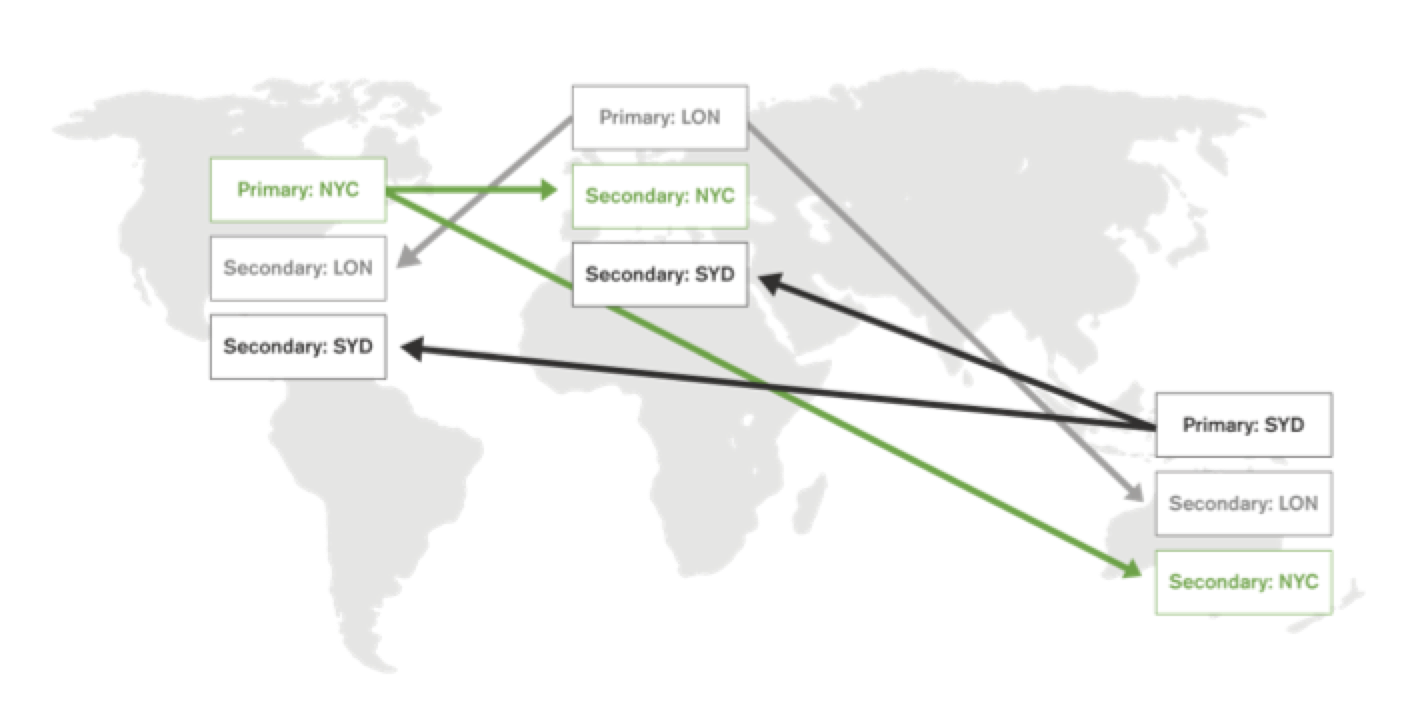
\includegraphics[width=\textwidth]{sources/MongoDB_sharded.png}\cite{MG10}
	\caption{Regionale Shards mit Replikatgruppen. Sekundärknoten befinden sich für niedrigere Latenzzeiten bei Lesezugriffen in anderen Regionen}
	\label{fig1}
\end{figure}

\paragraph{Fazit\\}
Beide Datenbanken liefern ausgereifte Methoden, um mit immer größer werdenden Datenmengen zurecht zu kommen. Für kleine bis mittlere Projekte sollten PostgreSQLs Skalierungsmöglichkeiten ausreichen, während sich große Projekte durch bessere Möglichkeiten des Shardings in MongoDB noch weiter Skalieren lassen. Auch scheint sich MongoDB mit weniger Arbeitsaufwand horizontal skalieren zu lassen, während bei PostgreSQL zuerst Anpassungen getätigt werden müssen. Damit ist MongoDB für dieses Projekt leicht präferiert.

\subsubsection{Hochverfügbarkeit}
Für den Anmeldevorgang, die Registrierung und alle Seiten unserer Plattform, die einen angemeldeten Nutzer voraussetzen, ist eine Datenbankanbindung zwingend erforderlich. Diese Teile machen den Großteil der Webseite aus, jede Minute, in der die Datenbank ausfällt, fällt unser Service nahezu komplett aus. Es bietet sich eine Datenbank mit Hochverfügbarkeit an, um das Risiko eines Ausfalls unserer Plattform so weit wie möglich zu verringern.\\
Um die Erreichbarkeit der Datenbank zu gewährleisten, bietet es sich an, Replikatgruppen zu erstellen. Eine Replikatgruppe besteht aus mehreren Datenbankprozessen, auch Knoten genannt, welche den gleichen Datensatz verwalten. Sollten durch Hardwarefehler einzelne Knoten ausfallen oder Softwarefehler Knoten dazu zwingen, neu gestartet zu werden, ist die Datenbank, wenn auch mit verringerter Leistung, weiterhin erreichbar. Die dadurch erreichte Fehlertoleranz schafft Sicherheit und verringert die Chance, dass die Datenbank komplett ausfällt drastisch.\\
Meist hat nur ein Prozess der Replikatgruppe Schreibrechte, um die Konsistenz bei gleichzeitigen Schreibzugriffen zu wahren. Neben diesem Primärknoten existieren oft mehrere Sekundärknoten, welche die Schreibvorgänge des Primärknotens kopieren und für Lesezugriffe zur Verfügung stehen. Es existieren andere Architekturen mit mehreren Primärknoten, die gleichzeitige Schreibzugriffe erlauben und besondere Herausforderungen bei der Datenkonsistenz stellen, diese werden hier jedoch nicht betrachtet.

\paragraph{}
PostgreSQL bietet verschiedene Lösungsansätze. Bei synchronen Lösungen muss ein Schreibauftrag von allen Knoten durchgeführt sein, um als bestätigt zu gelten. Asynchrone Lösungen erlauben einen Puffer zwischen dem Bestätigen eines Schreibauftrags und dessen Kopie auf andere Knoten, wodurch das Wechseln zu einem Backupknoten zu Datenverlust führen kann und Sekundärknoten bei Lesezugriffen ein leicht veraltertes Ergebnis liefern können. Dafür gewinnt eine asynchrone Lösung an Performanz, da sich die Wartezeit stark verringert; auch müssen die anderen Knoten seltener befragt und damit weniger belastet werden. Um die Knoten auf dem gleichen Stand zu halten und im Fall eines Ausfalls Daten wiederherstellen zu können, wird ein \textit{Write-Ahead Log} (WAL) angelegt, welcher unmittelbar nach jedem Commit die Transaktion in einen Transaktionslog schreibt. Dieser wird dann von anderen Knoten ausgelesen und die Transaktion wird kopiert. \cite{PG1}\\
Sollte der Primärknoten ausfallen, muss dies detektiert werden und ein Sekundärknoten mit so wenig Verzögerung wie möglich als neuer Primärknoten ausgewählt werden. PostgreSQL bietet keine automatische Ausfallsicherung, es muss daher eine Drittanbietersoftware verwendet werden oder ein eigener Skript geschrieben werden. Um die Belastung der einzelnen Knoten möglichst gleich zu halten, sollte ein Prozess zur Lastverteilung existieren. Den Recherchen nach bietet PostgreSQL selbst keine native Lastverteilung, daher werden Lösungen wie die kostenlose Open-Source Software HAProxy (High Availability Proxy) verwendet.

\paragraph{}
Knoten in MongoDBs Replikatgruppen teilen sich gegenseitig durch Ping-Befehle ihren \enquote{Herzschlag} mit, um zu ermitteln, ob ein Knoten ausgefallen ist. Sollte der Primärknoten \enquote{sterben}, wählen die \enquote{überlebenden} Knoten in einer Abstimmung den nächsten Primärknoten, welcher die Schreibaufträge des vorigen Primärknotens übernimmt. Der Prozess einer Wahl sollte in der Regel nicht länger als 12 Sekunden dauern und passiert vollautomatisch. Knoten mit mehr Leistung kann eine höhere Priorität zugewiesen werden, um diesen als präferierten Primärknoten zu definieren. Auch eignet es sich, Knoten in anderen Regionen für die Rolle des Primärknoten als unwählbar zu definieren, da sich die Latenz ansonsten drastisch erhöhen würde. Ein Replikset kann aus maximimal 50 Knoten bestehen, wovon bis zu 7 zum Primärknoten wählbar sind. \cite{MG3} \cite{MG4} Diese Zahl ist vermutlich groß genug, um einen gleichzeitigen Ausfall aller Knoten aus technischer Sicht nahezu unmöglich zu gestalten, wenn sich die Knoten zusätzlich auf verschiedenen physischen Geräten befinden.\\
In seltenen Fällen kann es vorkommen, dass der Primärknoten ausfällt und vor seinem Ausfall Schreibaufträge bestätigt, diese aber nicht an die Standbyknoten weiterleiten kann. Wenn der frühere Primärknoten der Replikatgruppe wieder beitritt, in diesem Fall als Sekundärknoten, unterscheidet sich dessen Schreibhistorie von der anderer Knoten. Die Historie des früheren Primärknoten wird zurückgerollt und die bestätigten Schreibaufträge sind verloren.\\
MongoDB versucht durch verschiedene Techniken, Rollbacks zu vermeiden und erlaubt es unter Verlust von Effizienz, mit Schreibbestätigungen erst zu antworten, wenn der Großteil der Replikatgruppe diese bestätigt hat. Sollte es trotzdem zu einem Rollback kommen, müssen einzelne Schreibaufträge oft manuell nach bestem Gewissen der Datenbankexperten wiederholt werden. \cite{MG5}\\
Leseanfragen werden per Standardkonfiguration an den Primärknoten gestellt, um möglichst aktuelle Daten liefern zu können. Diese Präferenz lässt sich ändern, um den Primärknoten zu entlasten, auf speziell eingerichtete Knoten mit optimisierten Indexen zugreifen zu können, die Latenz zu verringern oder beim Ausfall des Primärknotens weiterhin Lesezugriffe zu ermöglichen. Auch ist eine Wahl zwischen asynchronen und synchronen Operationen möglich, dabei sind asynchrone Operationen aufgrund der höheren Performanz die Standardeinstellung.

\paragraph{}
MongoDB überzeugt im Punkt der Hochverfügbarkeit gegenüber PostgreSQL. Um PostgreSQL hochverfügbar zu machen, sind einige Anpassungen und Expertenwissen oder Drittanbietersoftware nötig. MongoDB scheint von der Architektur auf Hochverfügbarkeit ausgerichtet zu sein und liefert Funktionen für eine automatische Ausfallsicherung, welche das System nach kurzer Zeit ohne manuelle Eingriffe wieder voll funktionstüchtig machen. Wir glauben, dass mit MongoDB eine Datenbank eingerichtet werden kann, die mit wenig Aufwand stabil für sehr geringe Ausfallraten sorgen kann.

\subsubsection{Dateiformat}
MongoDB speichert Daten im JSON-Format. JSON, die \enquote{JavaScript Object Notation}, ist \enquote{ein schlankes Datenaustauschformat, welches für Menschen einfach zu lesen und für Maschinen einfach zu parsen [] ist} \cite{JSON1}. JSON als semistrukturiertes Dateiformat eignet sich daher gut für Schnittstellendaten.\\
Desweiteren wird im gewählten MERN-Techstack ausschließlich JavaScript verwendet - das JavaScript native Dateiformat JSON ist daher ohne Umwandlungen direkt verwendbar und der Umgang für das Entwicklerteam bereits bekannt. Dies verringert die Gefahr möglicher Komplikationen und spart Lern- und Programmieraufwand. Diesen Vorteil besitzt PostgreSQL nicht, Abfrageergebnisse müssen für die Schnittstelle zuerst in JSON-Dateien geändert werden, was einen zusätzlichen Programmierschritt bedeutet. 

\subsubsection{Fazit}
\begin{center}
    \begin{tabularx}{\linewidth}{ |X|X|X| } 
        \hline
        Kriterien & PostgreSQL & MongoDB  \\ 
        \hline
        Lesegeschwindigkeit & Mittel & Hoch \\
        Schreibgeschwindigkeit & Mittel & Langsam - Mittel \\
        Datenstrukturen & Strenges Tabellenschema & Schemafrei durch Selbstbeschreibende JSON-Dokumente \\
        Skalierbarkeit & Meist vertikal, horizontal benötigt erweitertes Setup & Meist Horizontal, unterstützt nativ Sharding \\
        Hochverfügbarkeit & Replikatgruppen, Lastverteilung und automatische Ausfallsicherung meist über Drittsoftware & native Replikatgruppen und automatische Ausfallsicherung, Lastverteilung bei Wahl eines Sekundärknotens, automatische Wahl des nächsten Primärknotens bei Ausfall \\
        Dateiformat & internes Format, wird bei Abfragen in lesbaren Tabellen ausgegeben & JSON \\
        \hline
    \end{tabularx}
\end{center}

Es konnte gezeigt werden, dass beide Datenbanken eine ausgereifte Architektur besitzen und sich daher beide gut für Projekte eignen. Für dieses Projekt hat jedoch MongoDB einige Vorteile, die sich darauf zurückführen lassen, aus welchem Beweggrund MongoDB entstanden ist.\\
Die 2007 neu gegründete Firma 10Gen, mittlerweile bekannt als MongoDB Inc., benötigte eine Datenbank, welche den Anforderungen ihrer quelloffenen Plattform-as-a-Service Cloud-Architektur gerecht werden würde. Das Team suchte nach einer Datenbank, die elastisch, skalierbar, einfach zu verwalten und für Entwickler und Anwender einfach zu benutzen ist. Unzufrieden mit den zu der Zeit auf dem Markt verfügbaren Datenbanksystemen wurde MongoDB, eine dokumentbasierte Datenbank entwickelt. Als das Team das Potenzial der Datenbank realisierte, wurde die Idee der Cloud-Plattform eingestellt und die Entwicklung von MongoDB gefördert.\cite{MG9}\\
Aufgrund MongoDBs Historie sind automatische Ausfallsicherung, horizontale Skalierung und Sharding native Funktionen, die sich mit wenig Entwicklungsaufwand einstellen und skalieren lassen. Auf der Plattform ist es gut denkbar, dass auf einen komplexen Schreibzugriff dutzende, vielleicht hunderte Lesezugriffe kommen, die höhere Geschwindigkeit ist bemerkbar. Auch integriert sich das von MongoDB gewählte Dateiformat JSON gut mit der weiteren Architektur des verwendeten MERN-Techstacks.
Aus den genannten Gründen fällt die Wahl für das Projekt auf MongoDB.


\subsection{Schemata}
Folgende Kollektionen wurden verwendet, um die Daten optimal zu verwalten.

\paragraph{Nutzer}
\begin{center}
    \begin{tabularx}{\textwidth}{ |X|X|X| } 
     %\hline
     %Feld & Beschreibung & Beispiel \\ 
     %\hline
     % _id & Standardmäßige MongoId & \\
     % Benutzername & einzigartiger, öffentlicher Name & MaxMustermann \\ 
     % normalisierter Name & Name in Kleinbuchstaben. Wird verwendet, um die Einzigartigkeit von Namen zu gewährleisten & maxmustermann \\ 
     % Email & private eMail des Nutzers & mustermann@email.de \\
     % Rolle & Gibt an, ob der Nutzer autorisiert ist - Moderatoren und Administratorkonten haben mehr Rechte. Automatisch generiert & Nutzer \\ 
     % Geburtsdatum & privates Geburtsdatum des Nutzers & 01.01.2000 \\ 
     % Alter & Alter des Nutzers. Wird automatisch mit Geburtsdatum berechnet & 21 \\ 
     % Sprachen & Array von Sprachen, die der Nutzer sprechen kann & [de, en] \\
     % Geschlecht & gesellschaftliches Geschlecht des Nutzers. & Männlich \\ 
     % Spielposition & Bis zu 2 Lieblingspositionen des Spielers in League of Legends & [Mid, Jungle] \\ 
     % Freitext & kurzer Text, in dem der Nutzer sich beschreiben kann. & Ich bin ein toller Nutzer! \\
     % Avatar & URI [GLOSSAR!] vom Avatarbild des Nutzers & https://<s3-name>.s3.eu-central-1.amazonaws.com/avatars/<UUID>.jpg \\ 
     % Freunde & Array von allen Freunden des Nutzers. Beinhaltet die NutzerID und die ChatID & [[_id1, NutzerID1, ChatID1], [_id2, NutzerID2, ChatID2]]\\ 
     % Geblockt & Array von NutzerIDs der Nutzer, die geblockt wurden & [NutzerID3, NutzerID4] \\ 
     %\hline
    \end{tabularx}
\end{center}

Wenn ein Nutzer einen Account erstellt, gibt dieser dessen eMail, den gewünschten Benutzernamen und das gewünschte Passwort an. Durch Indexe wird die Einzigartigkeit von eMail und Benutzername geprüft, das Passwort wird aus Sicherheitsgründen in einer separaten Kollektion gespeichert. Nach der Kontoerstellung kann der Nutzer das Geburtsdatum, die gesprochenen Sprachen, das Geschlecht, die Spielposition und einen Freitext angeben und ein Bild hochladen, welches als Avatarbild dient. Felder wie der normalisierte Name, das Alter und die Rolle werden automatisch generiert. Im Laufe der Nutzung unserer Plattform wird der Nutzer andere Spieler als Freunde hinzufügen - diese werden in einer Freundesliste gespeichert. Auch steht es dem Nutzer frei, Andere zu blockieren - in diesem Fall wird die NutzerID des Blockierten auf die Blockliste hinzugefügt. \\
Privatsphäre und damit die Sicherheit der eigenen Daten stellt einen hohen Stellenwert dar. Die Anzahl an Daten, die ein Nutzer von sich preisgeben müssen, soll so gering wie möglich halten werden. Die Email-Adresse, das Geburtsdatum und Freundes- und Blockliste sind für andere Nutzer nicht einsehbar; bis auf den Benutzernamen, welcher einen Fantasienamen darstellen kann, muss eine Person keine Daten öffentlich angeben.

\paragraph{Sprache\\}
Damit Nutzer ihre gesprochenen Sprachen wählen können, bieten wir die Wahl zwischen 187 Sprachen nach ISO 639-1 Norm an.\cite{ISO639-1}\\

\begin{center}
    \begin{tabular}{ |c|c|c| }
        \hline
        Feld & Beschreibung & Beispiel \\
        \hline
        id & Alpha-2 Code der Sprache & en, de, fr \\
        name & Englische Schreibweise der Sprache & English, German, French \\
        nativer Name & native Schreibweise der Sprache & English, Deutsch, français \\
        \hline
    \end{tabular}
\end{center}
Standardmäßige Objekt-IDs von MongoDB enthalten einen Zeitstempel und einen inkrementellen Zähler.\cite{MG11} Diese Daten sind bei Sprachen - öffentlichen Stammdaten, die sich über einen langen Zeitraum nicht verändern werden - nicht relevant. Stattdessen wurde der Alpha-2-Code der Sprache als ID gewählt, der in den meisten Fällen auf die Sprache schließen lässt. Nutzerdokumente referenzieren die Sprache per ID. Dadurch stellt es kein großes Problem dar, direkt im Nutzerdokument anhand der Sprach-ID zu erkennen, welche Sprachen der Nutzer spricht. Fehler können einfacher vermieden werden und Tests sind einfacher menschlich nach Richtigkeit kontrollierbar.\\
Sprachen können sowohl anhand der englischen Schreibweise als auch der nativen Schreibweise gefunden werden. Dies erleichtert auch nicht-englischsprachigen Nutzern, ihre Sprache auswählen zu können.

\paragraph{Passwort\\}
\begin{center}
    \begin{tabular}{ |c|c| }
        \hline
        Feld & Beschreibung  \\
        \hline
        id & Standardmäßige MongoId \\
        password & Bcrypt Hash bestehend aus Versionsnummer, Komplexität, Salt und Hash \\
        NutzerID & MongoId des zugehörigen Nutzers \\
        \hline
    \end{tabular}
\end{center}

Das Passwort wird nicht im Nutzerdokument gespeichert. Wenn das Passwort im Nutzerdokument gespeichert werden würde, könnten schon kleine Programmierfehler dazu führen, dass normale Nutzer das gehashte Passwort anderer Nutzer ermitteln könnten. Um dieses Sicherheitsproblem direkt zu eliminieren, wird daher für jedes Passwort ein eigenes, vom Nutzerdokument isoliertes Dokument verwendet.\\
Das Passwort wird durch bcrypt, einem Blowfish-basiertem Hashalgorithmus, auf der Datenbank als Hash mit Salt gespeichert. Die Komplexität des Hashes frei wählbar. Bei der Wahl der Komplexität ist die Sicherheit gegen Rechengeschwindigkeit abzuwägen; eine höhere Komplexität erhöht die benötigte Zeit pro Versuch eines Angreifers, das Passwort zu knacken, erhöht gleichzeitig aber auch die Zeit, die unser Server benötigt, um ein neues Passwort zu generieren oder den Anmeldeversuch eines ehrlichen Nutzers zu bestätigen. Eine zu hohe Komplexität kann daher den Server stark verlangsamen und macht Angriffszenarien per (D)DOS ((distributed) denial of service, Überlastung des Servers durch übermäßigen Datenverkehr) gefährlicher, da gezielte Anmeldeversuche viel Last auf dem Server erzeugen. In Zukunft werden weitere Limitierungen auf Seiten des Backends erstellt, um wiederholte Anmeldeversuche zu bremsen.\\
Um die Wahrscheinlichkeit von Glückstreffern bei Angriffen zu verringern, wird verlangt, dass das Passwort mindestens aus 8 Zeichen, darunter 1 Großbuchstabe, 1 Kleinbuchstabe und 1 Ziffer erstellt wird. Für mehr Varianz in den Passwörtern sind zudem einige Sonderzeichen erlaubt. Durch gewählte Restriktionen besteht eine 1:1-Relation zwischen Passwörtern und Nutzerkonten.

\paragraph{Like\\}
\begin{center}
    \begin{tabular}{ |c|c| }
        \hline
        Feld & Beschreibung  \\
        \hline
        id & Standardmäßige MongoId \\
        Sender & NutzerID der Person, die den Like/Dislike versendet. \\
        Empfänger &  NutzerID der Person, die den Like/Dislike empfängt. \\
        Status & Gibt an, ob es sich um einen Like oder Dislike handelt. \\
        \hline
    \end{tabular}
\end{center}

\textit{Anmerkung: Der Name \enquote{Like} für diese Datenstruktur kann irreführend sein, da in der Kollektion sowohl Likes als auch Dislikes (angegeben durch den Status) gespeichert werden.\\}
Immer wenn ein Nutzer bei der Kontaktsuche angibt, ob er mit einer Person Kontakt aufnehmen oder diesen vermeiden will, wird ein Dokument angelegt. Wenn der Nutzer in Kontakt treten will, wird zusätzlich geprüft, ob bereits ein Datensatz existiert, bei dem Sender und Empfänger vertauscht sind - ob sich also die Nutzer gegenseitig einen Like gegeben haben. Sollte das der Fall sein, werden beide Datensätze gelöscht und die Nutzer zur Freundesliste des jeweils anderen hinzugefügt und ein Dokument der Kollektion Chat erstellt. in dem Fall können die Nutzer miteinander kommunizieren. Dislikes sorgen dafür, dass ein Kontakt in Zukunft nicht mehr möglich ist.

\paragraph{Chat\\}
\begin{center}
    \begin{tabular}{ |c|c| }
        \hline
        Feld & Beschreibung  \\
        \hline
        id & Standardmäßige MongoId \\
        Teilnehmer & Array von NutzerIDs, die dem Chat beiwohnen. Aktuell maximal 2. \\
        Nachrichten & Array von Nachrichten, die die Nutzer untereinander ausgetauscht haben. \\
        \hline
    \end{tabular}
\end{center}
Sollten sich zwei Nutzer befreunden, wird zwischen diesen ein Chat erstellt. Wenn ein Nutzer die Freundschaft beendet, verlässt dieser Nutzer gleichzeitig den Chat. Mit der gewählten Struktur sind auch Gruppenchats ohne Änderung der Datenbank möglich, falls dies in Zukunft eine erwünschte Funktion sein sollte.\\
Um Ressourcen zu sparen, wird bei der Standard-Datenbankabfrage nur die neueste Nachricht geladen. Diese Abfrage dient für Vorschaubilder des Chats in der Kontaktliste. Außerdem ist es möglich, durch Pagination (Seitennummerierung) je Abfrage 20 Nachrichten zu erfragen. Diese Methoden verringern die Serverlast, da in vielen Fällen nicht mehr als die erste Seite der Abfrage relevant ist.\\

\subparagraph{Nachricht\\}
Nachrichten sind eingebettete Dokumente eines Chats. Sie weisen folgende Datenstruktur auf.
\begin{center}
    \begin{tabular}{ |c|c| }
        \hline
        Feld & Beschreibung  \\
        \hline
        id & Standardmäßige MongoId \\
        Inhalt & Text der Nachricht \\
        Autor & NutzerID des Verfassers der Nachricht \\
        \hline
    \end{tabular}
\end{center}

\subsection{Database-as-a-Service}
Um eine Datenbank selbst zu betreiben fehlt es dem Projekt an fachlichen Kapazitäten und einer Infrastruktur, welche physische Datenbankserver unterstützt. Es bietet sich daher eine Database-as-a-Service-Lösung (DBaaS) an.\\ 
MongoDB Inc. bietet mit MongoDB Atlas eine DBaaS an, die flexibel auf die Größe und Auslastung des Projektes angepasst werden kann. Dazu gibt es verschiedene Datenbankstufen, die mit höheren Kosten mehr Rechenleistung und weitere Funktionen erhält. Zwischen den Stufen kann flexibel gewechselt werden, um den realen Auslastungen gerecht zu werden. Kostenpflichtige Stufen bieten die Möglichkeit an, Backups einzurichten, für höhere Kosten stehen Tools zur Verfügung, die Metriken in Echtzeit anzeigen, automatisch archivieren, Empfehlungen zur Leistungsoptimierung erstellen und langsame Datenbankabfragen zur Diagnose und Optimierung anzeigen. In der Entwicklungsphase wurde sich für die kostenlose Stufe entschieden, da die Funktionen und Leistung für die Entwicklungsumgebung ausreichen. Sollte das Produkt auf den Markt gehen, wird auf eine kostengünstigste Stufe gewechselt, um die Option von Backups zu erhalten. Sollte das Projekt erfolgreich sein und viele Nutzer anziehen, wird flexibel, abhängig von benötigter Leistung, eine teurere Stufe mit mehr Leistung gewählt.\\
Sowohl die Produktions-, als auch die Entwicklungsumgebung werden als eigene Datenbanken von MongoDB Atlas gehosted. Dies verringert das Risiko von Code, der auf der lokalen Maschine funktioniert, aber auf der Produktionsumgebung Fehler wirft. Durch die Nutzung gleicher Werkzeuge und gleicher Technologie wird die Werkzeuglücke verringert und dementsprechend die Dev-Prod-Vergleichbarkeit erhöht. \cite{12FA-10}

\subsection{Avatarbilder}
Statt Bilddateien für Avatare direkt auf der Datenbank zu speichern, was mit langen Wartezeiten auf die Datenbank einhergehen würde, werden nur die URIs zu den Bildern auf der Datenbank gespeichert. Für das Speichern der Binärdateien wurde sich für AWS S3 gehosted, einem Speichersystem, welches für BLOB-Dateien optimiert ist. Dies nimmt der Datenbank Last ab und erhöht die Anfragegeschwindigkeit bei Lese- und Schreibzugriffen des Avatarbildes.\\
Der S3-Speicher wurde so eingerichtet, dass das Backend Zugriffsrechte zum Erstellen und Löschen von Dateien hat. Beim Verteilen der Zugriffsrechte wurde nach Minimalprinzip vorgegangen, das Backend besitzt nur die Zugriffsrechte die es benötigt und keine weiteren. Ein möglicher Angriff verursacht dadurch weniger Schaden, als wenn das Backend alle Zugriffsrechte hätte.\\
Die Datenbank wird mithilfe von GraphQL angesprochen, für S3 hat sich diese Lösung jedoch nicht angeboten. Für das Hochladen von Profilbildern wurde eine weitere Route im Backend erstellt, bei der mit den npm-Packeten Multer und Multer-S3 kontrolliert wird, ob es sich bei der vom Nutzer hochgeladenen Datei um eine Bilddatei handelt und ob diese eine bestimmte Bildgröße nicht übersteigt.\\

\subsection{Fazit}
Mit den gewählten Kollektionen und der Wahl von speziellen Hosts sind wir in der Lage, Nutzern eine Datenbank anzubieten, die eine hohe Erreichbarkeit aufweist, sich leicht an die Auslastung skalieren lässt, personenbezogene Daten geheim hält und ein Maß an Datensicherheit bietet, welches der Größe des Projektes entspricht. Flexible Datenstrukturen erlauben schnelle Anpassungen des Projektes. Die Verwendung eines bekannten Dateiformats welches sich gut für Schnittstellen eignet sorgt für Zeitersparungen in der Entwicklung des Frontends und der Datenbankschnittstelle und reduziert somit den Aufwand. Außerdem werden durch eingebettete Dokumente, Denormalisierung und Seitennummerierung wurden Optimierungen durchgeführt, die als Ziel haben, möglichst schnell Antworten auf Leseanfragen zu bieten.